% Created by tikzDevice version 0.12.3 on 2020-05-24 19:40:55
% !TEX encoding = UTF-8 Unicode
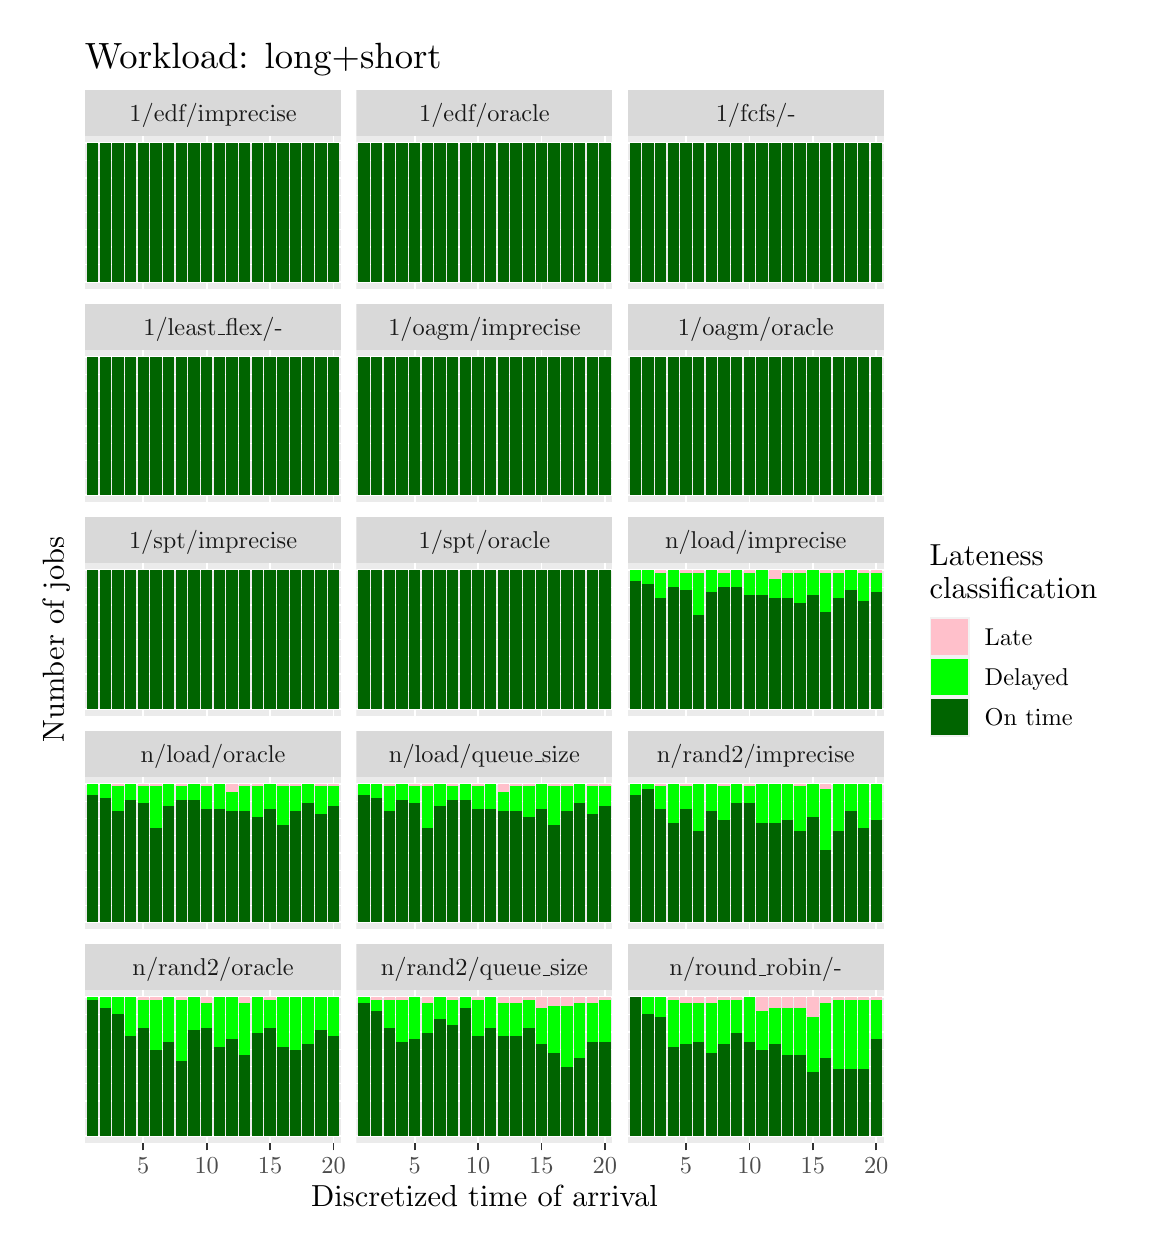
\begin{tikzpicture}[x=1pt,y=1pt]
\definecolor{fillColor}{RGB}{255,255,255}
\path[use as bounding box,fill=fillColor,fill opacity=0.00] (0,0) rectangle (397.48,433.62);
\begin{scope}
\path[clip] (  0.00,  0.00) rectangle (397.48,433.62);
\definecolor{drawColor}{RGB}{255,255,255}
\definecolor{fillColor}{RGB}{255,255,255}

\path[draw=drawColor,line width= 0.6pt,line join=round,line cap=round,fill=fillColor] (  0.00,  0.00) rectangle (397.48,433.62);
\end{scope}
\begin{scope}
\path[clip] ( 20.71,339.31) rectangle (113.27,394.39);
\definecolor{fillColor}{gray}{0.92}

\path[fill=fillColor] ( 20.71,339.31) rectangle (113.27,394.39);
\definecolor{drawColor}{RGB}{255,255,255}

\path[draw=drawColor,line width= 0.3pt,line join=round] ( 20.71,348.07) --
	(113.27,348.07);

\path[draw=drawColor,line width= 0.3pt,line join=round] ( 20.71,360.59) --
	(113.27,360.59);

\path[draw=drawColor,line width= 0.3pt,line join=round] ( 20.71,373.11) --
	(113.27,373.11);

\path[draw=drawColor,line width= 0.3pt,line join=round] ( 20.71,385.63) --
	(113.27,385.63);

\path[draw=drawColor,line width= 0.6pt,line join=round] ( 20.71,341.81) --
	(113.27,341.81);

\path[draw=drawColor,line width= 0.6pt,line join=round] ( 20.71,354.33) --
	(113.27,354.33);

\path[draw=drawColor,line width= 0.6pt,line join=round] ( 20.71,366.85) --
	(113.27,366.85);

\path[draw=drawColor,line width= 0.6pt,line join=round] ( 20.71,379.37) --
	(113.27,379.37);

\path[draw=drawColor,line width= 0.6pt,line join=round] ( 20.71,391.89) --
	(113.27,391.89);

\path[draw=drawColor,line width= 0.6pt,line join=round] ( 41.79,339.31) --
	( 41.79,394.39);

\path[draw=drawColor,line width= 0.6pt,line join=round] ( 64.70,339.31) --
	( 64.70,394.39);

\path[draw=drawColor,line width= 0.6pt,line join=round] ( 87.61,339.31) --
	( 87.61,394.39);

\path[draw=drawColor,line width= 0.6pt,line join=round] (110.52,339.31) --
	(110.52,394.39);
\definecolor{fillColor}{RGB}{0,100,0}

\path[fill=fillColor] ( 21.40,341.81) rectangle ( 25.53,391.89);

\path[fill=fillColor] ( 25.98,341.81) rectangle ( 30.11,391.89);

\path[fill=fillColor] ( 30.57,341.81) rectangle ( 34.69,391.89);

\path[fill=fillColor] ( 35.15,341.81) rectangle ( 39.27,391.89);

\path[fill=fillColor] ( 39.73,341.81) rectangle ( 43.85,391.89);

\path[fill=fillColor] ( 44.31,341.81) rectangle ( 48.43,391.89);

\path[fill=fillColor] ( 48.89,341.81) rectangle ( 53.02,391.89);

\path[fill=fillColor] ( 53.47,341.81) rectangle ( 57.60,391.89);

\path[fill=fillColor] ( 58.06,341.81) rectangle ( 62.18,391.89);

\path[fill=fillColor] ( 62.64,341.81) rectangle ( 66.76,391.89);

\path[fill=fillColor] ( 67.22,341.81) rectangle ( 71.34,391.89);

\path[fill=fillColor] ( 71.80,341.81) rectangle ( 75.93,391.89);

\path[fill=fillColor] ( 76.38,341.81) rectangle ( 80.51,391.89);

\path[fill=fillColor] ( 80.97,341.81) rectangle ( 85.09,391.89);

\path[fill=fillColor] ( 85.55,341.81) rectangle ( 89.67,391.89);

\path[fill=fillColor] ( 90.13,341.81) rectangle ( 94.25,391.89);

\path[fill=fillColor] ( 94.71,341.81) rectangle ( 98.84,391.89);

\path[fill=fillColor] ( 99.29,341.81) rectangle (103.42,391.89);

\path[fill=fillColor] (103.88,341.81) rectangle (108.00,391.89);

\path[fill=fillColor] (108.46,341.81) rectangle (112.58,391.89);
\end{scope}
\begin{scope}
\path[clip] ( 20.71,262.15) rectangle (113.27,317.24);
\definecolor{fillColor}{gray}{0.92}

\path[fill=fillColor] ( 20.71,262.15) rectangle (113.27,317.24);
\definecolor{drawColor}{RGB}{255,255,255}

\path[draw=drawColor,line width= 0.3pt,line join=round] ( 20.71,270.92) --
	(113.27,270.92);

\path[draw=drawColor,line width= 0.3pt,line join=round] ( 20.71,283.43) --
	(113.27,283.43);

\path[draw=drawColor,line width= 0.3pt,line join=round] ( 20.71,295.95) --
	(113.27,295.95);

\path[draw=drawColor,line width= 0.3pt,line join=round] ( 20.71,308.47) --
	(113.27,308.47);

\path[draw=drawColor,line width= 0.6pt,line join=round] ( 20.71,264.66) --
	(113.27,264.66);

\path[draw=drawColor,line width= 0.6pt,line join=round] ( 20.71,277.17) --
	(113.27,277.17);

\path[draw=drawColor,line width= 0.6pt,line join=round] ( 20.71,289.69) --
	(113.27,289.69);

\path[draw=drawColor,line width= 0.6pt,line join=round] ( 20.71,302.21) --
	(113.27,302.21);

\path[draw=drawColor,line width= 0.6pt,line join=round] ( 20.71,314.73) --
	(113.27,314.73);

\path[draw=drawColor,line width= 0.6pt,line join=round] ( 41.79,262.15) --
	( 41.79,317.24);

\path[draw=drawColor,line width= 0.6pt,line join=round] ( 64.70,262.15) --
	( 64.70,317.24);

\path[draw=drawColor,line width= 0.6pt,line join=round] ( 87.61,262.15) --
	( 87.61,317.24);

\path[draw=drawColor,line width= 0.6pt,line join=round] (110.52,262.15) --
	(110.52,317.24);
\definecolor{fillColor}{RGB}{0,100,0}

\path[fill=fillColor] ( 21.40,264.66) rectangle ( 25.53,314.73);

\path[fill=fillColor] ( 25.98,264.66) rectangle ( 30.11,314.73);

\path[fill=fillColor] ( 30.57,264.66) rectangle ( 34.69,314.73);

\path[fill=fillColor] ( 35.15,264.66) rectangle ( 39.27,314.73);

\path[fill=fillColor] ( 39.73,264.66) rectangle ( 43.85,314.73);

\path[fill=fillColor] ( 44.31,264.66) rectangle ( 48.43,314.73);

\path[fill=fillColor] ( 48.89,264.66) rectangle ( 53.02,314.73);

\path[fill=fillColor] ( 53.47,264.66) rectangle ( 57.60,314.73);

\path[fill=fillColor] ( 58.06,264.66) rectangle ( 62.18,314.73);

\path[fill=fillColor] ( 62.64,264.66) rectangle ( 66.76,314.73);

\path[fill=fillColor] ( 67.22,264.66) rectangle ( 71.34,314.73);

\path[fill=fillColor] ( 71.80,264.66) rectangle ( 75.93,314.73);

\path[fill=fillColor] ( 76.38,264.66) rectangle ( 80.51,314.73);

\path[fill=fillColor] ( 80.97,264.66) rectangle ( 85.09,314.73);

\path[fill=fillColor] ( 85.55,264.66) rectangle ( 89.67,314.73);

\path[fill=fillColor] ( 90.13,264.66) rectangle ( 94.25,314.73);

\path[fill=fillColor] ( 94.71,264.66) rectangle ( 98.84,314.73);

\path[fill=fillColor] ( 99.29,264.66) rectangle (103.42,314.73);

\path[fill=fillColor] (103.88,264.66) rectangle (108.00,314.73);

\path[fill=fillColor] (108.46,264.66) rectangle (112.58,314.73);
\end{scope}
\begin{scope}
\path[clip] ( 20.71,185.00) rectangle (113.27,240.08);
\definecolor{fillColor}{gray}{0.92}

\path[fill=fillColor] ( 20.71,185.00) rectangle (113.27,240.08);
\definecolor{drawColor}{RGB}{255,255,255}

\path[draw=drawColor,line width= 0.3pt,line join=round] ( 20.71,193.76) --
	(113.27,193.76);

\path[draw=drawColor,line width= 0.3pt,line join=round] ( 20.71,206.28) --
	(113.27,206.28);

\path[draw=drawColor,line width= 0.3pt,line join=round] ( 20.71,218.80) --
	(113.27,218.80);

\path[draw=drawColor,line width= 0.3pt,line join=round] ( 20.71,231.32) --
	(113.27,231.32);

\path[draw=drawColor,line width= 0.6pt,line join=round] ( 20.71,187.50) --
	(113.27,187.50);

\path[draw=drawColor,line width= 0.6pt,line join=round] ( 20.71,200.02) --
	(113.27,200.02);

\path[draw=drawColor,line width= 0.6pt,line join=round] ( 20.71,212.54) --
	(113.27,212.54);

\path[draw=drawColor,line width= 0.6pt,line join=round] ( 20.71,225.06) --
	(113.27,225.06);

\path[draw=drawColor,line width= 0.6pt,line join=round] ( 20.71,237.58) --
	(113.27,237.58);

\path[draw=drawColor,line width= 0.6pt,line join=round] ( 41.79,185.00) --
	( 41.79,240.08);

\path[draw=drawColor,line width= 0.6pt,line join=round] ( 64.70,185.00) --
	( 64.70,240.08);

\path[draw=drawColor,line width= 0.6pt,line join=round] ( 87.61,185.00) --
	( 87.61,240.08);

\path[draw=drawColor,line width= 0.6pt,line join=round] (110.52,185.00) --
	(110.52,240.08);
\definecolor{fillColor}{RGB}{0,100,0}

\path[fill=fillColor] ( 21.40,187.50) rectangle ( 25.53,237.58);

\path[fill=fillColor] ( 25.98,187.50) rectangle ( 30.11,237.58);

\path[fill=fillColor] ( 30.57,187.50) rectangle ( 34.69,237.58);

\path[fill=fillColor] ( 35.15,187.50) rectangle ( 39.27,237.58);

\path[fill=fillColor] ( 39.73,187.50) rectangle ( 43.85,237.58);

\path[fill=fillColor] ( 44.31,187.50) rectangle ( 48.43,237.58);

\path[fill=fillColor] ( 48.89,187.50) rectangle ( 53.02,237.58);

\path[fill=fillColor] ( 53.47,187.50) rectangle ( 57.60,237.58);

\path[fill=fillColor] ( 58.06,187.50) rectangle ( 62.18,237.58);

\path[fill=fillColor] ( 62.64,187.50) rectangle ( 66.76,237.58);

\path[fill=fillColor] ( 67.22,187.50) rectangle ( 71.34,237.58);

\path[fill=fillColor] ( 71.80,187.50) rectangle ( 75.93,237.58);

\path[fill=fillColor] ( 76.38,187.50) rectangle ( 80.51,237.58);

\path[fill=fillColor] ( 80.97,187.50) rectangle ( 85.09,237.58);

\path[fill=fillColor] ( 85.55,187.50) rectangle ( 89.67,237.58);

\path[fill=fillColor] ( 90.13,187.50) rectangle ( 94.25,237.58);

\path[fill=fillColor] ( 94.71,187.50) rectangle ( 98.84,237.58);

\path[fill=fillColor] ( 99.29,187.50) rectangle (103.42,237.58);

\path[fill=fillColor] (103.88,187.50) rectangle (108.00,237.58);

\path[fill=fillColor] (108.46,187.50) rectangle (112.58,237.58);
\end{scope}
\begin{scope}
\path[clip] ( 20.71,107.84) rectangle (113.27,162.93);
\definecolor{fillColor}{gray}{0.92}

\path[fill=fillColor] ( 20.71,107.84) rectangle (113.27,162.93);
\definecolor{drawColor}{RGB}{255,255,255}

\path[draw=drawColor,line width= 0.3pt,line join=round] ( 20.71,116.60) --
	(113.27,116.60);

\path[draw=drawColor,line width= 0.3pt,line join=round] ( 20.71,129.12) --
	(113.27,129.12);

\path[draw=drawColor,line width= 0.3pt,line join=round] ( 20.71,141.64) --
	(113.27,141.64);

\path[draw=drawColor,line width= 0.3pt,line join=round] ( 20.71,154.16) --
	(113.27,154.16);

\path[draw=drawColor,line width= 0.6pt,line join=round] ( 20.71,110.35) --
	(113.27,110.35);

\path[draw=drawColor,line width= 0.6pt,line join=round] ( 20.71,122.86) --
	(113.27,122.86);

\path[draw=drawColor,line width= 0.6pt,line join=round] ( 20.71,135.38) --
	(113.27,135.38);

\path[draw=drawColor,line width= 0.6pt,line join=round] ( 20.71,147.90) --
	(113.27,147.90);

\path[draw=drawColor,line width= 0.6pt,line join=round] ( 20.71,160.42) --
	(113.27,160.42);

\path[draw=drawColor,line width= 0.6pt,line join=round] ( 41.79,107.84) --
	( 41.79,162.93);

\path[draw=drawColor,line width= 0.6pt,line join=round] ( 64.70,107.84) --
	( 64.70,162.93);

\path[draw=drawColor,line width= 0.6pt,line join=round] ( 87.61,107.84) --
	( 87.61,162.93);

\path[draw=drawColor,line width= 0.6pt,line join=round] (110.52,107.84) --
	(110.52,162.93);
\definecolor{fillColor}{RGB}{255,192,203}

\path[fill=fillColor] ( 30.57,159.42) rectangle ( 34.69,160.42);

\path[fill=fillColor] ( 39.73,159.42) rectangle ( 43.85,160.42);

\path[fill=fillColor] ( 44.31,159.42) rectangle ( 48.43,160.42);

\path[fill=fillColor] ( 53.47,159.42) rectangle ( 57.60,160.42);

\path[fill=fillColor] ( 62.64,159.42) rectangle ( 66.76,160.42);

\path[fill=fillColor] ( 71.80,157.42) rectangle ( 75.93,160.42);

\path[fill=fillColor] ( 76.38,159.42) rectangle ( 80.51,160.42);

\path[fill=fillColor] ( 80.97,159.42) rectangle ( 85.09,160.42);

\path[fill=fillColor] ( 90.13,159.42) rectangle ( 94.25,160.42);

\path[fill=fillColor] ( 94.71,159.42) rectangle ( 98.84,160.42);

\path[fill=fillColor] (103.88,159.42) rectangle (108.00,160.42);

\path[fill=fillColor] (108.46,159.42) rectangle (112.58,160.42);
\definecolor{fillColor}{RGB}{0,255,0}

\path[fill=fillColor] ( 21.40,156.42) rectangle ( 25.53,160.42);

\path[fill=fillColor] ( 25.98,155.41) rectangle ( 30.11,160.42);

\path[fill=fillColor] ( 30.57,150.41) rectangle ( 34.69,159.42);

\path[fill=fillColor] ( 35.15,154.41) rectangle ( 39.27,160.42);

\path[fill=fillColor] ( 39.73,153.41) rectangle ( 43.85,159.42);

\path[fill=fillColor] ( 44.31,144.40) rectangle ( 48.43,159.42);

\path[fill=fillColor] ( 48.89,152.41) rectangle ( 53.02,160.42);

\path[fill=fillColor] ( 53.47,154.41) rectangle ( 57.60,159.42);

\path[fill=fillColor] ( 58.06,154.41) rectangle ( 62.18,160.42);

\path[fill=fillColor] ( 62.64,151.41) rectangle ( 66.76,159.42);

\path[fill=fillColor] ( 67.22,151.41) rectangle ( 71.34,160.42);

\path[fill=fillColor] ( 71.80,150.41) rectangle ( 75.93,157.42);

\path[fill=fillColor] ( 76.38,150.41) rectangle ( 80.51,159.42);

\path[fill=fillColor] ( 80.97,148.40) rectangle ( 85.09,159.42);

\path[fill=fillColor] ( 85.55,151.41) rectangle ( 89.67,160.42);

\path[fill=fillColor] ( 90.13,145.40) rectangle ( 94.25,159.42);

\path[fill=fillColor] ( 94.71,150.41) rectangle ( 98.84,159.42);

\path[fill=fillColor] ( 99.29,153.41) rectangle (103.42,160.42);

\path[fill=fillColor] (103.88,149.40) rectangle (108.00,159.42);

\path[fill=fillColor] (108.46,152.41) rectangle (112.58,159.42);
\definecolor{fillColor}{RGB}{0,100,0}

\path[fill=fillColor] ( 21.40,110.35) rectangle ( 25.53,156.42);

\path[fill=fillColor] ( 25.98,110.35) rectangle ( 30.11,155.41);

\path[fill=fillColor] ( 30.57,110.35) rectangle ( 34.69,150.41);

\path[fill=fillColor] ( 35.15,110.35) rectangle ( 39.27,154.41);

\path[fill=fillColor] ( 39.73,110.35) rectangle ( 43.85,153.41);

\path[fill=fillColor] ( 44.31,110.35) rectangle ( 48.43,144.40);

\path[fill=fillColor] ( 48.89,110.35) rectangle ( 53.02,152.41);

\path[fill=fillColor] ( 53.47,110.35) rectangle ( 57.60,154.41);

\path[fill=fillColor] ( 58.06,110.35) rectangle ( 62.18,154.41);

\path[fill=fillColor] ( 62.64,110.35) rectangle ( 66.76,151.41);

\path[fill=fillColor] ( 67.22,110.35) rectangle ( 71.34,151.41);

\path[fill=fillColor] ( 71.80,110.35) rectangle ( 75.93,150.41);

\path[fill=fillColor] ( 76.38,110.35) rectangle ( 80.51,150.41);

\path[fill=fillColor] ( 80.97,110.35) rectangle ( 85.09,148.40);

\path[fill=fillColor] ( 85.55,110.35) rectangle ( 89.67,151.41);

\path[fill=fillColor] ( 90.13,110.35) rectangle ( 94.25,145.40);

\path[fill=fillColor] ( 94.71,110.35) rectangle ( 98.84,150.41);

\path[fill=fillColor] ( 99.29,110.35) rectangle (103.42,153.41);

\path[fill=fillColor] (103.88,110.35) rectangle (108.00,149.40);

\path[fill=fillColor] (108.46,110.35) rectangle (112.58,152.41);
\end{scope}
\begin{scope}
\path[clip] ( 20.71, 30.69) rectangle (113.27, 85.77);
\definecolor{fillColor}{gray}{0.92}

\path[fill=fillColor] ( 20.71, 30.69) rectangle (113.27, 85.77);
\definecolor{drawColor}{RGB}{255,255,255}

\path[draw=drawColor,line width= 0.3pt,line join=round] ( 20.71, 39.45) --
	(113.27, 39.45);

\path[draw=drawColor,line width= 0.3pt,line join=round] ( 20.71, 51.97) --
	(113.27, 51.97);

\path[draw=drawColor,line width= 0.3pt,line join=round] ( 20.71, 64.49) --
	(113.27, 64.49);

\path[draw=drawColor,line width= 0.3pt,line join=round] ( 20.71, 77.01) --
	(113.27, 77.01);

\path[draw=drawColor,line width= 0.6pt,line join=round] ( 20.71, 33.19) --
	(113.27, 33.19);

\path[draw=drawColor,line width= 0.6pt,line join=round] ( 20.71, 45.71) --
	(113.27, 45.71);

\path[draw=drawColor,line width= 0.6pt,line join=round] ( 20.71, 58.23) --
	(113.27, 58.23);

\path[draw=drawColor,line width= 0.6pt,line join=round] ( 20.71, 70.75) --
	(113.27, 70.75);

\path[draw=drawColor,line width= 0.6pt,line join=round] ( 20.71, 83.27) --
	(113.27, 83.27);

\path[draw=drawColor,line width= 0.6pt,line join=round] ( 41.79, 30.69) --
	( 41.79, 85.77);

\path[draw=drawColor,line width= 0.6pt,line join=round] ( 64.70, 30.69) --
	( 64.70, 85.77);

\path[draw=drawColor,line width= 0.6pt,line join=round] ( 87.61, 30.69) --
	( 87.61, 85.77);

\path[draw=drawColor,line width= 0.6pt,line join=round] (110.52, 30.69) --
	(110.52, 85.77);
\definecolor{fillColor}{RGB}{255,192,203}

\path[fill=fillColor] ( 39.73, 82.26) rectangle ( 43.85, 83.27);

\path[fill=fillColor] ( 44.31, 82.26) rectangle ( 48.43, 83.27);

\path[fill=fillColor] ( 53.47, 82.26) rectangle ( 57.60, 83.27);

\path[fill=fillColor] ( 62.64, 81.26) rectangle ( 66.76, 83.27);

\path[fill=fillColor] ( 76.38, 81.26) rectangle ( 80.51, 83.27);

\path[fill=fillColor] ( 85.55, 82.26) rectangle ( 89.67, 83.27);
\definecolor{fillColor}{RGB}{0,255,0}

\path[fill=fillColor] ( 21.40, 82.26) rectangle ( 25.53, 83.27);

\path[fill=fillColor] ( 25.98, 79.26) rectangle ( 30.11, 83.27);

\path[fill=fillColor] ( 30.57, 77.26) rectangle ( 34.69, 83.27);

\path[fill=fillColor] ( 35.15, 69.24) rectangle ( 39.27, 83.27);

\path[fill=fillColor] ( 39.73, 72.25) rectangle ( 43.85, 82.26);

\path[fill=fillColor] ( 44.31, 64.24) rectangle ( 48.43, 82.26);

\path[fill=fillColor] ( 48.89, 67.24) rectangle ( 53.02, 83.27);

\path[fill=fillColor] ( 53.47, 60.23) rectangle ( 57.60, 82.26);

\path[fill=fillColor] ( 58.06, 71.25) rectangle ( 62.18, 83.27);

\path[fill=fillColor] ( 62.64, 72.25) rectangle ( 66.76, 81.26);

\path[fill=fillColor] ( 67.22, 65.24) rectangle ( 71.34, 83.27);

\path[fill=fillColor] ( 71.80, 68.24) rectangle ( 75.93, 83.27);

\path[fill=fillColor] ( 76.38, 62.23) rectangle ( 80.51, 81.26);

\path[fill=fillColor] ( 80.97, 70.25) rectangle ( 85.09, 83.27);

\path[fill=fillColor] ( 85.55, 72.25) rectangle ( 89.67, 82.26);

\path[fill=fillColor] ( 90.13, 65.24) rectangle ( 94.25, 83.27);

\path[fill=fillColor] ( 94.71, 64.24) rectangle ( 98.84, 83.27);

\path[fill=fillColor] ( 99.29, 66.24) rectangle (103.42, 83.27);

\path[fill=fillColor] (103.88, 71.25) rectangle (108.00, 83.27);

\path[fill=fillColor] (108.46, 69.24) rectangle (112.58, 83.27);
\definecolor{fillColor}{RGB}{0,100,0}

\path[fill=fillColor] ( 21.40, 33.19) rectangle ( 25.53, 82.26);

\path[fill=fillColor] ( 25.98, 33.19) rectangle ( 30.11, 79.26);

\path[fill=fillColor] ( 30.57, 33.19) rectangle ( 34.69, 77.26);

\path[fill=fillColor] ( 35.15, 33.19) rectangle ( 39.27, 69.24);

\path[fill=fillColor] ( 39.73, 33.19) rectangle ( 43.85, 72.25);

\path[fill=fillColor] ( 44.31, 33.19) rectangle ( 48.43, 64.24);

\path[fill=fillColor] ( 48.89, 33.19) rectangle ( 53.02, 67.24);

\path[fill=fillColor] ( 53.47, 33.19) rectangle ( 57.60, 60.23);

\path[fill=fillColor] ( 58.06, 33.19) rectangle ( 62.18, 71.25);

\path[fill=fillColor] ( 62.64, 33.19) rectangle ( 66.76, 72.25);

\path[fill=fillColor] ( 67.22, 33.19) rectangle ( 71.34, 65.24);

\path[fill=fillColor] ( 71.80, 33.19) rectangle ( 75.93, 68.24);

\path[fill=fillColor] ( 76.38, 33.19) rectangle ( 80.51, 62.23);

\path[fill=fillColor] ( 80.97, 33.19) rectangle ( 85.09, 70.25);

\path[fill=fillColor] ( 85.55, 33.19) rectangle ( 89.67, 72.25);

\path[fill=fillColor] ( 90.13, 33.19) rectangle ( 94.25, 65.24);

\path[fill=fillColor] ( 94.71, 33.19) rectangle ( 98.84, 64.24);

\path[fill=fillColor] ( 99.29, 33.19) rectangle (103.42, 66.24);

\path[fill=fillColor] (103.88, 33.19) rectangle (108.00, 71.25);

\path[fill=fillColor] (108.46, 33.19) rectangle (112.58, 69.24);
\end{scope}
\begin{scope}
\path[clip] (118.77,339.31) rectangle (211.32,394.39);
\definecolor{fillColor}{gray}{0.92}

\path[fill=fillColor] (118.77,339.31) rectangle (211.32,394.39);
\definecolor{drawColor}{RGB}{255,255,255}

\path[draw=drawColor,line width= 0.3pt,line join=round] (118.77,348.07) --
	(211.32,348.07);

\path[draw=drawColor,line width= 0.3pt,line join=round] (118.77,360.59) --
	(211.32,360.59);

\path[draw=drawColor,line width= 0.3pt,line join=round] (118.77,373.11) --
	(211.32,373.11);

\path[draw=drawColor,line width= 0.3pt,line join=round] (118.77,385.63) --
	(211.32,385.63);

\path[draw=drawColor,line width= 0.6pt,line join=round] (118.77,341.81) --
	(211.32,341.81);

\path[draw=drawColor,line width= 0.6pt,line join=round] (118.77,354.33) --
	(211.32,354.33);

\path[draw=drawColor,line width= 0.6pt,line join=round] (118.77,366.85) --
	(211.32,366.85);

\path[draw=drawColor,line width= 0.6pt,line join=round] (118.77,379.37) --
	(211.32,379.37);

\path[draw=drawColor,line width= 0.6pt,line join=round] (118.77,391.89) --
	(211.32,391.89);

\path[draw=drawColor,line width= 0.6pt,line join=round] (139.85,339.31) --
	(139.85,394.39);

\path[draw=drawColor,line width= 0.6pt,line join=round] (162.75,339.31) --
	(162.75,394.39);

\path[draw=drawColor,line width= 0.6pt,line join=round] (185.66,339.31) --
	(185.66,394.39);

\path[draw=drawColor,line width= 0.6pt,line join=round] (208.57,339.31) --
	(208.57,394.39);
\definecolor{fillColor}{RGB}{0,100,0}

\path[fill=fillColor] (119.46,341.81) rectangle (123.58,391.89);

\path[fill=fillColor] (124.04,341.81) rectangle (128.16,391.89);

\path[fill=fillColor] (128.62,341.81) rectangle (132.74,391.89);

\path[fill=fillColor] (133.20,341.81) rectangle (137.33,391.89);

\path[fill=fillColor] (137.78,341.81) rectangle (141.91,391.89);

\path[fill=fillColor] (142.37,341.81) rectangle (146.49,391.89);

\path[fill=fillColor] (146.95,341.81) rectangle (151.07,391.89);

\path[fill=fillColor] (151.53,341.81) rectangle (155.65,391.89);

\path[fill=fillColor] (156.11,341.81) rectangle (160.23,391.89);

\path[fill=fillColor] (160.69,341.81) rectangle (164.82,391.89);

\path[fill=fillColor] (165.27,341.81) rectangle (169.40,391.89);

\path[fill=fillColor] (169.86,341.81) rectangle (173.98,391.89);

\path[fill=fillColor] (174.44,341.81) rectangle (178.56,391.89);

\path[fill=fillColor] (179.02,341.81) rectangle (183.14,391.89);

\path[fill=fillColor] (183.60,341.81) rectangle (187.73,391.89);

\path[fill=fillColor] (188.18,341.81) rectangle (192.31,391.89);

\path[fill=fillColor] (192.77,341.81) rectangle (196.89,391.89);

\path[fill=fillColor] (197.35,341.81) rectangle (201.47,391.89);

\path[fill=fillColor] (201.93,341.81) rectangle (206.05,391.89);

\path[fill=fillColor] (206.51,341.81) rectangle (210.64,391.89);
\end{scope}
\begin{scope}
\path[clip] (118.77,262.15) rectangle (211.32,317.24);
\definecolor{fillColor}{gray}{0.92}

\path[fill=fillColor] (118.77,262.15) rectangle (211.32,317.24);
\definecolor{drawColor}{RGB}{255,255,255}

\path[draw=drawColor,line width= 0.3pt,line join=round] (118.77,270.92) --
	(211.32,270.92);

\path[draw=drawColor,line width= 0.3pt,line join=round] (118.77,283.43) --
	(211.32,283.43);

\path[draw=drawColor,line width= 0.3pt,line join=round] (118.77,295.95) --
	(211.32,295.95);

\path[draw=drawColor,line width= 0.3pt,line join=round] (118.77,308.47) --
	(211.32,308.47);

\path[draw=drawColor,line width= 0.6pt,line join=round] (118.77,264.66) --
	(211.32,264.66);

\path[draw=drawColor,line width= 0.6pt,line join=round] (118.77,277.17) --
	(211.32,277.17);

\path[draw=drawColor,line width= 0.6pt,line join=round] (118.77,289.69) --
	(211.32,289.69);

\path[draw=drawColor,line width= 0.6pt,line join=round] (118.77,302.21) --
	(211.32,302.21);

\path[draw=drawColor,line width= 0.6pt,line join=round] (118.77,314.73) --
	(211.32,314.73);

\path[draw=drawColor,line width= 0.6pt,line join=round] (139.85,262.15) --
	(139.85,317.24);

\path[draw=drawColor,line width= 0.6pt,line join=round] (162.75,262.15) --
	(162.75,317.24);

\path[draw=drawColor,line width= 0.6pt,line join=round] (185.66,262.15) --
	(185.66,317.24);

\path[draw=drawColor,line width= 0.6pt,line join=round] (208.57,262.15) --
	(208.57,317.24);
\definecolor{fillColor}{RGB}{0,100,0}

\path[fill=fillColor] (119.46,264.66) rectangle (123.58,314.73);

\path[fill=fillColor] (124.04,264.66) rectangle (128.16,314.73);

\path[fill=fillColor] (128.62,264.66) rectangle (132.74,314.73);

\path[fill=fillColor] (133.20,264.66) rectangle (137.33,314.73);

\path[fill=fillColor] (137.78,264.66) rectangle (141.91,314.73);

\path[fill=fillColor] (142.37,264.66) rectangle (146.49,314.73);

\path[fill=fillColor] (146.95,264.66) rectangle (151.07,314.73);

\path[fill=fillColor] (151.53,264.66) rectangle (155.65,314.73);

\path[fill=fillColor] (156.11,264.66) rectangle (160.23,314.73);

\path[fill=fillColor] (160.69,264.66) rectangle (164.82,314.73);

\path[fill=fillColor] (165.27,264.66) rectangle (169.40,314.73);

\path[fill=fillColor] (169.86,264.66) rectangle (173.98,314.73);

\path[fill=fillColor] (174.44,264.66) rectangle (178.56,314.73);

\path[fill=fillColor] (179.02,264.66) rectangle (183.14,314.73);

\path[fill=fillColor] (183.60,264.66) rectangle (187.73,314.73);

\path[fill=fillColor] (188.18,264.66) rectangle (192.31,314.73);

\path[fill=fillColor] (192.77,264.66) rectangle (196.89,314.73);

\path[fill=fillColor] (197.35,264.66) rectangle (201.47,314.73);

\path[fill=fillColor] (201.93,264.66) rectangle (206.05,314.73);

\path[fill=fillColor] (206.51,264.66) rectangle (210.64,314.73);
\end{scope}
\begin{scope}
\path[clip] (118.77,185.00) rectangle (211.32,240.08);
\definecolor{fillColor}{gray}{0.92}

\path[fill=fillColor] (118.77,185.00) rectangle (211.32,240.08);
\definecolor{drawColor}{RGB}{255,255,255}

\path[draw=drawColor,line width= 0.3pt,line join=round] (118.77,193.76) --
	(211.32,193.76);

\path[draw=drawColor,line width= 0.3pt,line join=round] (118.77,206.28) --
	(211.32,206.28);

\path[draw=drawColor,line width= 0.3pt,line join=round] (118.77,218.80) --
	(211.32,218.80);

\path[draw=drawColor,line width= 0.3pt,line join=round] (118.77,231.32) --
	(211.32,231.32);

\path[draw=drawColor,line width= 0.6pt,line join=round] (118.77,187.50) --
	(211.32,187.50);

\path[draw=drawColor,line width= 0.6pt,line join=round] (118.77,200.02) --
	(211.32,200.02);

\path[draw=drawColor,line width= 0.6pt,line join=round] (118.77,212.54) --
	(211.32,212.54);

\path[draw=drawColor,line width= 0.6pt,line join=round] (118.77,225.06) --
	(211.32,225.06);

\path[draw=drawColor,line width= 0.6pt,line join=round] (118.77,237.58) --
	(211.32,237.58);

\path[draw=drawColor,line width= 0.6pt,line join=round] (139.85,185.00) --
	(139.85,240.08);

\path[draw=drawColor,line width= 0.6pt,line join=round] (162.75,185.00) --
	(162.75,240.08);

\path[draw=drawColor,line width= 0.6pt,line join=round] (185.66,185.00) --
	(185.66,240.08);

\path[draw=drawColor,line width= 0.6pt,line join=round] (208.57,185.00) --
	(208.57,240.08);
\definecolor{fillColor}{RGB}{0,100,0}

\path[fill=fillColor] (119.46,187.50) rectangle (123.58,237.58);

\path[fill=fillColor] (124.04,187.50) rectangle (128.16,237.58);

\path[fill=fillColor] (128.62,187.50) rectangle (132.74,237.58);

\path[fill=fillColor] (133.20,187.50) rectangle (137.33,237.58);

\path[fill=fillColor] (137.78,187.50) rectangle (141.91,237.58);

\path[fill=fillColor] (142.37,187.50) rectangle (146.49,237.58);

\path[fill=fillColor] (146.95,187.50) rectangle (151.07,237.58);

\path[fill=fillColor] (151.53,187.50) rectangle (155.65,237.58);

\path[fill=fillColor] (156.11,187.50) rectangle (160.23,237.58);

\path[fill=fillColor] (160.69,187.50) rectangle (164.82,237.58);

\path[fill=fillColor] (165.27,187.50) rectangle (169.40,237.58);

\path[fill=fillColor] (169.86,187.50) rectangle (173.98,237.58);

\path[fill=fillColor] (174.44,187.50) rectangle (178.56,237.58);

\path[fill=fillColor] (179.02,187.50) rectangle (183.14,237.58);

\path[fill=fillColor] (183.60,187.50) rectangle (187.73,237.58);

\path[fill=fillColor] (188.18,187.50) rectangle (192.31,237.58);

\path[fill=fillColor] (192.77,187.50) rectangle (196.89,237.58);

\path[fill=fillColor] (197.35,187.50) rectangle (201.47,237.58);

\path[fill=fillColor] (201.93,187.50) rectangle (206.05,237.58);

\path[fill=fillColor] (206.51,187.50) rectangle (210.64,237.58);
\end{scope}
\begin{scope}
\path[clip] (118.77,107.84) rectangle (211.32,162.93);
\definecolor{fillColor}{gray}{0.92}

\path[fill=fillColor] (118.77,107.84) rectangle (211.32,162.93);
\definecolor{drawColor}{RGB}{255,255,255}

\path[draw=drawColor,line width= 0.3pt,line join=round] (118.77,116.60) --
	(211.32,116.60);

\path[draw=drawColor,line width= 0.3pt,line join=round] (118.77,129.12) --
	(211.32,129.12);

\path[draw=drawColor,line width= 0.3pt,line join=round] (118.77,141.64) --
	(211.32,141.64);

\path[draw=drawColor,line width= 0.3pt,line join=round] (118.77,154.16) --
	(211.32,154.16);

\path[draw=drawColor,line width= 0.6pt,line join=round] (118.77,110.35) --
	(211.32,110.35);

\path[draw=drawColor,line width= 0.6pt,line join=round] (118.77,122.86) --
	(211.32,122.86);

\path[draw=drawColor,line width= 0.6pt,line join=round] (118.77,135.38) --
	(211.32,135.38);

\path[draw=drawColor,line width= 0.6pt,line join=round] (118.77,147.90) --
	(211.32,147.90);

\path[draw=drawColor,line width= 0.6pt,line join=round] (118.77,160.42) --
	(211.32,160.42);

\path[draw=drawColor,line width= 0.6pt,line join=round] (139.85,107.84) --
	(139.85,162.93);

\path[draw=drawColor,line width= 0.6pt,line join=round] (162.75,107.84) --
	(162.75,162.93);

\path[draw=drawColor,line width= 0.6pt,line join=round] (185.66,107.84) --
	(185.66,162.93);

\path[draw=drawColor,line width= 0.6pt,line join=round] (208.57,107.84) --
	(208.57,162.93);
\definecolor{fillColor}{RGB}{255,192,203}

\path[fill=fillColor] (128.62,159.42) rectangle (132.74,160.42);

\path[fill=fillColor] (137.78,159.42) rectangle (141.91,160.42);

\path[fill=fillColor] (142.37,159.42) rectangle (146.49,160.42);

\path[fill=fillColor] (151.53,159.42) rectangle (155.65,160.42);

\path[fill=fillColor] (160.69,159.42) rectangle (164.82,160.42);

\path[fill=fillColor] (169.86,157.42) rectangle (173.98,160.42);

\path[fill=fillColor] (174.44,159.42) rectangle (178.56,160.42);

\path[fill=fillColor] (179.02,159.42) rectangle (183.14,160.42);

\path[fill=fillColor] (188.18,159.42) rectangle (192.31,160.42);

\path[fill=fillColor] (192.77,159.42) rectangle (196.89,160.42);

\path[fill=fillColor] (201.93,159.42) rectangle (206.05,160.42);

\path[fill=fillColor] (206.51,159.42) rectangle (210.64,160.42);
\definecolor{fillColor}{RGB}{0,255,0}

\path[fill=fillColor] (119.46,156.42) rectangle (123.58,160.42);

\path[fill=fillColor] (124.04,155.41) rectangle (128.16,160.42);

\path[fill=fillColor] (128.62,150.41) rectangle (132.74,159.42);

\path[fill=fillColor] (133.20,154.41) rectangle (137.33,160.42);

\path[fill=fillColor] (137.78,153.41) rectangle (141.91,159.42);

\path[fill=fillColor] (142.37,144.40) rectangle (146.49,159.42);

\path[fill=fillColor] (146.95,152.41) rectangle (151.07,160.42);

\path[fill=fillColor] (151.53,154.41) rectangle (155.65,159.42);

\path[fill=fillColor] (156.11,154.41) rectangle (160.23,160.42);

\path[fill=fillColor] (160.69,151.41) rectangle (164.82,159.42);

\path[fill=fillColor] (165.27,151.41) rectangle (169.40,160.42);

\path[fill=fillColor] (169.86,150.41) rectangle (173.98,157.42);

\path[fill=fillColor] (174.44,150.41) rectangle (178.56,159.42);

\path[fill=fillColor] (179.02,148.40) rectangle (183.14,159.42);

\path[fill=fillColor] (183.60,151.41) rectangle (187.73,160.42);

\path[fill=fillColor] (188.18,145.40) rectangle (192.31,159.42);

\path[fill=fillColor] (192.77,150.41) rectangle (196.89,159.42);

\path[fill=fillColor] (197.35,153.41) rectangle (201.47,160.42);

\path[fill=fillColor] (201.93,149.40) rectangle (206.05,159.42);

\path[fill=fillColor] (206.51,152.41) rectangle (210.64,159.42);
\definecolor{fillColor}{RGB}{0,100,0}

\path[fill=fillColor] (119.46,110.35) rectangle (123.58,156.42);

\path[fill=fillColor] (124.04,110.35) rectangle (128.16,155.41);

\path[fill=fillColor] (128.62,110.35) rectangle (132.74,150.41);

\path[fill=fillColor] (133.20,110.35) rectangle (137.33,154.41);

\path[fill=fillColor] (137.78,110.35) rectangle (141.91,153.41);

\path[fill=fillColor] (142.37,110.35) rectangle (146.49,144.40);

\path[fill=fillColor] (146.95,110.35) rectangle (151.07,152.41);

\path[fill=fillColor] (151.53,110.35) rectangle (155.65,154.41);

\path[fill=fillColor] (156.11,110.35) rectangle (160.23,154.41);

\path[fill=fillColor] (160.69,110.35) rectangle (164.82,151.41);

\path[fill=fillColor] (165.27,110.35) rectangle (169.40,151.41);

\path[fill=fillColor] (169.86,110.35) rectangle (173.98,150.41);

\path[fill=fillColor] (174.44,110.35) rectangle (178.56,150.41);

\path[fill=fillColor] (179.02,110.35) rectangle (183.14,148.40);

\path[fill=fillColor] (183.60,110.35) rectangle (187.73,151.41);

\path[fill=fillColor] (188.18,110.35) rectangle (192.31,145.40);

\path[fill=fillColor] (192.77,110.35) rectangle (196.89,150.41);

\path[fill=fillColor] (197.35,110.35) rectangle (201.47,153.41);

\path[fill=fillColor] (201.93,110.35) rectangle (206.05,149.40);

\path[fill=fillColor] (206.51,110.35) rectangle (210.64,152.41);
\end{scope}
\begin{scope}
\path[clip] (118.77, 30.69) rectangle (211.32, 85.77);
\definecolor{fillColor}{gray}{0.92}

\path[fill=fillColor] (118.77, 30.69) rectangle (211.32, 85.77);
\definecolor{drawColor}{RGB}{255,255,255}

\path[draw=drawColor,line width= 0.3pt,line join=round] (118.77, 39.45) --
	(211.32, 39.45);

\path[draw=drawColor,line width= 0.3pt,line join=round] (118.77, 51.97) --
	(211.32, 51.97);

\path[draw=drawColor,line width= 0.3pt,line join=round] (118.77, 64.49) --
	(211.32, 64.49);

\path[draw=drawColor,line width= 0.3pt,line join=round] (118.77, 77.01) --
	(211.32, 77.01);

\path[draw=drawColor,line width= 0.6pt,line join=round] (118.77, 33.19) --
	(211.32, 33.19);

\path[draw=drawColor,line width= 0.6pt,line join=round] (118.77, 45.71) --
	(211.32, 45.71);

\path[draw=drawColor,line width= 0.6pt,line join=round] (118.77, 58.23) --
	(211.32, 58.23);

\path[draw=drawColor,line width= 0.6pt,line join=round] (118.77, 70.75) --
	(211.32, 70.75);

\path[draw=drawColor,line width= 0.6pt,line join=round] (118.77, 83.27) --
	(211.32, 83.27);

\path[draw=drawColor,line width= 0.6pt,line join=round] (139.85, 30.69) --
	(139.85, 85.77);

\path[draw=drawColor,line width= 0.6pt,line join=round] (162.75, 30.69) --
	(162.75, 85.77);

\path[draw=drawColor,line width= 0.6pt,line join=round] (185.66, 30.69) --
	(185.66, 85.77);

\path[draw=drawColor,line width= 0.6pt,line join=round] (208.57, 30.69) --
	(208.57, 85.77);
\definecolor{fillColor}{RGB}{255,192,203}

\path[fill=fillColor] (124.04, 82.26) rectangle (128.16, 83.27);

\path[fill=fillColor] (128.62, 82.26) rectangle (132.74, 83.27);

\path[fill=fillColor] (133.20, 82.26) rectangle (137.33, 83.27);

\path[fill=fillColor] (142.37, 81.26) rectangle (146.49, 83.27);

\path[fill=fillColor] (151.53, 82.26) rectangle (155.65, 83.27);

\path[fill=fillColor] (160.69, 82.26) rectangle (164.82, 83.27);

\path[fill=fillColor] (169.86, 81.26) rectangle (173.98, 83.27);

\path[fill=fillColor] (174.44, 81.26) rectangle (178.56, 83.27);

\path[fill=fillColor] (179.02, 82.26) rectangle (183.14, 83.27);

\path[fill=fillColor] (183.60, 79.26) rectangle (187.73, 83.27);

\path[fill=fillColor] (188.18, 80.26) rectangle (192.31, 83.27);

\path[fill=fillColor] (192.77, 80.26) rectangle (196.89, 83.27);

\path[fill=fillColor] (197.35, 81.26) rectangle (201.47, 83.27);

\path[fill=fillColor] (201.93, 81.26) rectangle (206.05, 83.27);

\path[fill=fillColor] (206.51, 82.26) rectangle (210.64, 83.27);
\definecolor{fillColor}{RGB}{0,255,0}

\path[fill=fillColor] (119.46, 81.26) rectangle (123.58, 83.27);

\path[fill=fillColor] (124.04, 78.26) rectangle (128.16, 82.26);

\path[fill=fillColor] (128.62, 72.25) rectangle (132.74, 82.26);

\path[fill=fillColor] (133.20, 67.24) rectangle (137.33, 82.26);

\path[fill=fillColor] (137.78, 68.24) rectangle (141.91, 83.27);

\path[fill=fillColor] (142.37, 70.25) rectangle (146.49, 81.26);

\path[fill=fillColor] (146.95, 75.25) rectangle (151.07, 83.27);

\path[fill=fillColor] (151.53, 73.25) rectangle (155.65, 82.26);

\path[fill=fillColor] (156.11, 79.26) rectangle (160.23, 83.27);

\path[fill=fillColor] (160.69, 69.24) rectangle (164.82, 82.26);

\path[fill=fillColor] (165.27, 72.25) rectangle (169.40, 83.27);

\path[fill=fillColor] (169.86, 69.24) rectangle (173.98, 81.26);

\path[fill=fillColor] (174.44, 69.24) rectangle (178.56, 81.26);

\path[fill=fillColor] (179.02, 72.25) rectangle (183.14, 82.26);

\path[fill=fillColor] (183.60, 66.24) rectangle (187.73, 79.26);

\path[fill=fillColor] (188.18, 63.24) rectangle (192.31, 80.26);

\path[fill=fillColor] (192.77, 58.23) rectangle (196.89, 80.26);

\path[fill=fillColor] (197.35, 61.23) rectangle (201.47, 81.26);

\path[fill=fillColor] (201.93, 67.24) rectangle (206.05, 81.26);

\path[fill=fillColor] (206.51, 67.24) rectangle (210.64, 82.26);
\definecolor{fillColor}{RGB}{0,100,0}

\path[fill=fillColor] (119.46, 33.19) rectangle (123.58, 81.26);

\path[fill=fillColor] (124.04, 33.19) rectangle (128.16, 78.26);

\path[fill=fillColor] (128.62, 33.19) rectangle (132.74, 72.25);

\path[fill=fillColor] (133.20, 33.19) rectangle (137.33, 67.24);

\path[fill=fillColor] (137.78, 33.19) rectangle (141.91, 68.24);

\path[fill=fillColor] (142.37, 33.19) rectangle (146.49, 70.25);

\path[fill=fillColor] (146.95, 33.19) rectangle (151.07, 75.25);

\path[fill=fillColor] (151.53, 33.19) rectangle (155.65, 73.25);

\path[fill=fillColor] (156.11, 33.19) rectangle (160.23, 79.26);

\path[fill=fillColor] (160.69, 33.19) rectangle (164.82, 69.24);

\path[fill=fillColor] (165.27, 33.19) rectangle (169.40, 72.25);

\path[fill=fillColor] (169.86, 33.19) rectangle (173.98, 69.24);

\path[fill=fillColor] (174.44, 33.19) rectangle (178.56, 69.24);

\path[fill=fillColor] (179.02, 33.19) rectangle (183.14, 72.25);

\path[fill=fillColor] (183.60, 33.19) rectangle (187.73, 66.24);

\path[fill=fillColor] (188.18, 33.19) rectangle (192.31, 63.24);

\path[fill=fillColor] (192.77, 33.19) rectangle (196.89, 58.23);

\path[fill=fillColor] (197.35, 33.19) rectangle (201.47, 61.23);

\path[fill=fillColor] (201.93, 33.19) rectangle (206.05, 67.24);

\path[fill=fillColor] (206.51, 33.19) rectangle (210.64, 67.24);
\end{scope}
\begin{scope}
\path[clip] (216.82,339.31) rectangle (309.38,394.39);
\definecolor{fillColor}{gray}{0.92}

\path[fill=fillColor] (216.82,339.31) rectangle (309.38,394.39);
\definecolor{drawColor}{RGB}{255,255,255}

\path[draw=drawColor,line width= 0.3pt,line join=round] (216.82,348.07) --
	(309.38,348.07);

\path[draw=drawColor,line width= 0.3pt,line join=round] (216.82,360.59) --
	(309.38,360.59);

\path[draw=drawColor,line width= 0.3pt,line join=round] (216.82,373.11) --
	(309.38,373.11);

\path[draw=drawColor,line width= 0.3pt,line join=round] (216.82,385.63) --
	(309.38,385.63);

\path[draw=drawColor,line width= 0.6pt,line join=round] (216.82,341.81) --
	(309.38,341.81);

\path[draw=drawColor,line width= 0.6pt,line join=round] (216.82,354.33) --
	(309.38,354.33);

\path[draw=drawColor,line width= 0.6pt,line join=round] (216.82,366.85) --
	(309.38,366.85);

\path[draw=drawColor,line width= 0.6pt,line join=round] (216.82,379.37) --
	(309.38,379.37);

\path[draw=drawColor,line width= 0.6pt,line join=round] (216.82,391.89) --
	(309.38,391.89);

\path[draw=drawColor,line width= 0.6pt,line join=round] (237.90,339.31) --
	(237.90,394.39);

\path[draw=drawColor,line width= 0.6pt,line join=round] (260.81,339.31) --
	(260.81,394.39);

\path[draw=drawColor,line width= 0.6pt,line join=round] (283.72,339.31) --
	(283.72,394.39);

\path[draw=drawColor,line width= 0.6pt,line join=round] (306.63,339.31) --
	(306.63,394.39);
\definecolor{fillColor}{RGB}{0,100,0}

\path[fill=fillColor] (217.51,341.81) rectangle (221.63,391.89);

\path[fill=fillColor] (222.09,341.81) rectangle (226.22,391.89);

\path[fill=fillColor] (226.67,341.81) rectangle (230.80,391.89);

\path[fill=fillColor] (231.26,341.81) rectangle (235.38,391.89);

\path[fill=fillColor] (235.84,341.81) rectangle (239.96,391.89);

\path[fill=fillColor] (240.42,341.81) rectangle (244.54,391.89);

\path[fill=fillColor] (245.00,341.81) rectangle (249.13,391.89);

\path[fill=fillColor] (249.58,341.81) rectangle (253.71,391.89);

\path[fill=fillColor] (254.17,341.81) rectangle (258.29,391.89);

\path[fill=fillColor] (258.75,341.81) rectangle (262.87,391.89);

\path[fill=fillColor] (263.33,341.81) rectangle (267.45,391.89);

\path[fill=fillColor] (267.91,341.81) rectangle (272.03,391.89);

\path[fill=fillColor] (272.49,341.81) rectangle (276.62,391.89);

\path[fill=fillColor] (277.07,341.81) rectangle (281.20,391.89);

\path[fill=fillColor] (281.66,341.81) rectangle (285.78,391.89);

\path[fill=fillColor] (286.24,341.81) rectangle (290.36,391.89);

\path[fill=fillColor] (290.82,341.81) rectangle (294.94,391.89);

\path[fill=fillColor] (295.40,341.81) rectangle (299.53,391.89);

\path[fill=fillColor] (299.98,341.81) rectangle (304.11,391.89);

\path[fill=fillColor] (304.57,341.81) rectangle (308.69,391.89);
\end{scope}
\begin{scope}
\path[clip] (216.82,262.15) rectangle (309.38,317.24);
\definecolor{fillColor}{gray}{0.92}

\path[fill=fillColor] (216.82,262.15) rectangle (309.38,317.24);
\definecolor{drawColor}{RGB}{255,255,255}

\path[draw=drawColor,line width= 0.3pt,line join=round] (216.82,270.92) --
	(309.38,270.92);

\path[draw=drawColor,line width= 0.3pt,line join=round] (216.82,283.43) --
	(309.38,283.43);

\path[draw=drawColor,line width= 0.3pt,line join=round] (216.82,295.95) --
	(309.38,295.95);

\path[draw=drawColor,line width= 0.3pt,line join=round] (216.82,308.47) --
	(309.38,308.47);

\path[draw=drawColor,line width= 0.6pt,line join=round] (216.82,264.66) --
	(309.38,264.66);

\path[draw=drawColor,line width= 0.6pt,line join=round] (216.82,277.17) --
	(309.38,277.17);

\path[draw=drawColor,line width= 0.6pt,line join=round] (216.82,289.69) --
	(309.38,289.69);

\path[draw=drawColor,line width= 0.6pt,line join=round] (216.82,302.21) --
	(309.38,302.21);

\path[draw=drawColor,line width= 0.6pt,line join=round] (216.82,314.73) --
	(309.38,314.73);

\path[draw=drawColor,line width= 0.6pt,line join=round] (237.90,262.15) --
	(237.90,317.24);

\path[draw=drawColor,line width= 0.6pt,line join=round] (260.81,262.15) --
	(260.81,317.24);

\path[draw=drawColor,line width= 0.6pt,line join=round] (283.72,262.15) --
	(283.72,317.24);

\path[draw=drawColor,line width= 0.6pt,line join=round] (306.63,262.15) --
	(306.63,317.24);
\definecolor{fillColor}{RGB}{0,100,0}

\path[fill=fillColor] (217.51,264.66) rectangle (221.63,314.73);

\path[fill=fillColor] (222.09,264.66) rectangle (226.22,314.73);

\path[fill=fillColor] (226.67,264.66) rectangle (230.80,314.73);

\path[fill=fillColor] (231.26,264.66) rectangle (235.38,314.73);

\path[fill=fillColor] (235.84,264.66) rectangle (239.96,314.73);

\path[fill=fillColor] (240.42,264.66) rectangle (244.54,314.73);

\path[fill=fillColor] (245.00,264.66) rectangle (249.13,314.73);

\path[fill=fillColor] (249.58,264.66) rectangle (253.71,314.73);

\path[fill=fillColor] (254.17,264.66) rectangle (258.29,314.73);

\path[fill=fillColor] (258.75,264.66) rectangle (262.87,314.73);

\path[fill=fillColor] (263.33,264.66) rectangle (267.45,314.73);

\path[fill=fillColor] (267.91,264.66) rectangle (272.03,314.73);

\path[fill=fillColor] (272.49,264.66) rectangle (276.62,314.73);

\path[fill=fillColor] (277.07,264.66) rectangle (281.20,314.73);

\path[fill=fillColor] (281.66,264.66) rectangle (285.78,314.73);

\path[fill=fillColor] (286.24,264.66) rectangle (290.36,314.73);

\path[fill=fillColor] (290.82,264.66) rectangle (294.94,314.73);

\path[fill=fillColor] (295.40,264.66) rectangle (299.53,314.73);

\path[fill=fillColor] (299.98,264.66) rectangle (304.11,314.73);

\path[fill=fillColor] (304.57,264.66) rectangle (308.69,314.73);
\end{scope}
\begin{scope}
\path[clip] (216.82,185.00) rectangle (309.38,240.08);
\definecolor{fillColor}{gray}{0.92}

\path[fill=fillColor] (216.82,185.00) rectangle (309.38,240.08);
\definecolor{drawColor}{RGB}{255,255,255}

\path[draw=drawColor,line width= 0.3pt,line join=round] (216.82,193.76) --
	(309.38,193.76);

\path[draw=drawColor,line width= 0.3pt,line join=round] (216.82,206.28) --
	(309.38,206.28);

\path[draw=drawColor,line width= 0.3pt,line join=round] (216.82,218.80) --
	(309.38,218.80);

\path[draw=drawColor,line width= 0.3pt,line join=round] (216.82,231.32) --
	(309.38,231.32);

\path[draw=drawColor,line width= 0.6pt,line join=round] (216.82,187.50) --
	(309.38,187.50);

\path[draw=drawColor,line width= 0.6pt,line join=round] (216.82,200.02) --
	(309.38,200.02);

\path[draw=drawColor,line width= 0.6pt,line join=round] (216.82,212.54) --
	(309.38,212.54);

\path[draw=drawColor,line width= 0.6pt,line join=round] (216.82,225.06) --
	(309.38,225.06);

\path[draw=drawColor,line width= 0.6pt,line join=round] (216.82,237.58) --
	(309.38,237.58);

\path[draw=drawColor,line width= 0.6pt,line join=round] (237.90,185.00) --
	(237.90,240.08);

\path[draw=drawColor,line width= 0.6pt,line join=round] (260.81,185.00) --
	(260.81,240.08);

\path[draw=drawColor,line width= 0.6pt,line join=round] (283.72,185.00) --
	(283.72,240.08);

\path[draw=drawColor,line width= 0.6pt,line join=round] (306.63,185.00) --
	(306.63,240.08);
\definecolor{fillColor}{RGB}{255,192,203}

\path[fill=fillColor] (226.67,236.58) rectangle (230.80,237.58);

\path[fill=fillColor] (235.84,236.58) rectangle (239.96,237.58);

\path[fill=fillColor] (240.42,236.58) rectangle (244.54,237.58);

\path[fill=fillColor] (249.58,236.58) rectangle (253.71,237.58);

\path[fill=fillColor] (258.75,236.58) rectangle (262.87,237.58);

\path[fill=fillColor] (267.91,234.57) rectangle (272.03,237.58);

\path[fill=fillColor] (272.49,236.58) rectangle (276.62,237.58);

\path[fill=fillColor] (277.07,236.58) rectangle (281.20,237.58);

\path[fill=fillColor] (286.24,236.58) rectangle (290.36,237.58);

\path[fill=fillColor] (290.82,236.58) rectangle (294.94,237.58);

\path[fill=fillColor] (299.98,236.58) rectangle (304.11,237.58);

\path[fill=fillColor] (304.57,236.58) rectangle (308.69,237.58);
\definecolor{fillColor}{RGB}{0,255,0}

\path[fill=fillColor] (217.51,233.57) rectangle (221.63,237.58);

\path[fill=fillColor] (222.09,232.57) rectangle (226.22,237.58);

\path[fill=fillColor] (226.67,227.56) rectangle (230.80,236.58);

\path[fill=fillColor] (231.26,231.57) rectangle (235.38,237.58);

\path[fill=fillColor] (235.84,230.57) rectangle (239.96,236.58);

\path[fill=fillColor] (240.42,221.55) rectangle (244.54,236.58);

\path[fill=fillColor] (245.00,229.56) rectangle (249.13,237.58);

\path[fill=fillColor] (249.58,231.57) rectangle (253.71,236.58);

\path[fill=fillColor] (254.17,231.57) rectangle (258.29,237.58);

\path[fill=fillColor] (258.75,228.56) rectangle (262.87,236.58);

\path[fill=fillColor] (263.33,228.56) rectangle (267.45,237.58);

\path[fill=fillColor] (267.91,227.56) rectangle (272.03,234.57);

\path[fill=fillColor] (272.49,227.56) rectangle (276.62,236.58);

\path[fill=fillColor] (277.07,225.56) rectangle (281.20,236.58);

\path[fill=fillColor] (281.66,228.56) rectangle (285.78,237.58);

\path[fill=fillColor] (286.24,222.55) rectangle (290.36,236.58);

\path[fill=fillColor] (290.82,227.56) rectangle (294.94,236.58);

\path[fill=fillColor] (295.40,230.57) rectangle (299.53,237.58);

\path[fill=fillColor] (299.98,226.56) rectangle (304.11,236.58);

\path[fill=fillColor] (304.57,229.56) rectangle (308.69,236.58);
\definecolor{fillColor}{RGB}{0,100,0}

\path[fill=fillColor] (217.51,187.50) rectangle (221.63,233.57);

\path[fill=fillColor] (222.09,187.50) rectangle (226.22,232.57);

\path[fill=fillColor] (226.67,187.50) rectangle (230.80,227.56);

\path[fill=fillColor] (231.26,187.50) rectangle (235.38,231.57);

\path[fill=fillColor] (235.84,187.50) rectangle (239.96,230.57);

\path[fill=fillColor] (240.42,187.50) rectangle (244.54,221.55);

\path[fill=fillColor] (245.00,187.50) rectangle (249.13,229.56);

\path[fill=fillColor] (249.58,187.50) rectangle (253.71,231.57);

\path[fill=fillColor] (254.17,187.50) rectangle (258.29,231.57);

\path[fill=fillColor] (258.75,187.50) rectangle (262.87,228.56);

\path[fill=fillColor] (263.33,187.50) rectangle (267.45,228.56);

\path[fill=fillColor] (267.91,187.50) rectangle (272.03,227.56);

\path[fill=fillColor] (272.49,187.50) rectangle (276.62,227.56);

\path[fill=fillColor] (277.07,187.50) rectangle (281.20,225.56);

\path[fill=fillColor] (281.66,187.50) rectangle (285.78,228.56);

\path[fill=fillColor] (286.24,187.50) rectangle (290.36,222.55);

\path[fill=fillColor] (290.82,187.50) rectangle (294.94,227.56);

\path[fill=fillColor] (295.40,187.50) rectangle (299.53,230.57);

\path[fill=fillColor] (299.98,187.50) rectangle (304.11,226.56);

\path[fill=fillColor] (304.57,187.50) rectangle (308.69,229.56);
\end{scope}
\begin{scope}
\path[clip] (216.82,107.84) rectangle (309.38,162.93);
\definecolor{fillColor}{gray}{0.92}

\path[fill=fillColor] (216.82,107.84) rectangle (309.38,162.93);
\definecolor{drawColor}{RGB}{255,255,255}

\path[draw=drawColor,line width= 0.3pt,line join=round] (216.82,116.60) --
	(309.38,116.60);

\path[draw=drawColor,line width= 0.3pt,line join=round] (216.82,129.12) --
	(309.38,129.12);

\path[draw=drawColor,line width= 0.3pt,line join=round] (216.82,141.64) --
	(309.38,141.64);

\path[draw=drawColor,line width= 0.3pt,line join=round] (216.82,154.16) --
	(309.38,154.16);

\path[draw=drawColor,line width= 0.6pt,line join=round] (216.82,110.35) --
	(309.38,110.35);

\path[draw=drawColor,line width= 0.6pt,line join=round] (216.82,122.86) --
	(309.38,122.86);

\path[draw=drawColor,line width= 0.6pt,line join=round] (216.82,135.38) --
	(309.38,135.38);

\path[draw=drawColor,line width= 0.6pt,line join=round] (216.82,147.90) --
	(309.38,147.90);

\path[draw=drawColor,line width= 0.6pt,line join=round] (216.82,160.42) --
	(309.38,160.42);

\path[draw=drawColor,line width= 0.6pt,line join=round] (237.90,107.84) --
	(237.90,162.93);

\path[draw=drawColor,line width= 0.6pt,line join=round] (260.81,107.84) --
	(260.81,162.93);

\path[draw=drawColor,line width= 0.6pt,line join=round] (283.72,107.84) --
	(283.72,162.93);

\path[draw=drawColor,line width= 0.6pt,line join=round] (306.63,107.84) --
	(306.63,162.93);
\definecolor{fillColor}{RGB}{255,192,203}

\path[fill=fillColor] (226.67,159.42) rectangle (230.80,160.42);

\path[fill=fillColor] (235.84,159.42) rectangle (239.96,160.42);

\path[fill=fillColor] (249.58,159.42) rectangle (253.71,160.42);

\path[fill=fillColor] (258.75,159.42) rectangle (262.87,160.42);

\path[fill=fillColor] (277.07,159.42) rectangle (281.20,160.42);

\path[fill=fillColor] (286.24,158.42) rectangle (290.36,160.42);
\definecolor{fillColor}{RGB}{0,255,0}

\path[fill=fillColor] (217.51,156.42) rectangle (221.63,160.42);

\path[fill=fillColor] (222.09,158.42) rectangle (226.22,160.42);

\path[fill=fillColor] (226.67,151.41) rectangle (230.80,159.42);

\path[fill=fillColor] (231.26,146.40) rectangle (235.38,160.42);

\path[fill=fillColor] (235.84,151.41) rectangle (239.96,159.42);

\path[fill=fillColor] (240.42,143.40) rectangle (244.54,160.42);

\path[fill=fillColor] (245.00,150.41) rectangle (249.13,160.42);

\path[fill=fillColor] (249.58,147.40) rectangle (253.71,159.42);

\path[fill=fillColor] (254.17,153.41) rectangle (258.29,160.42);

\path[fill=fillColor] (258.75,153.41) rectangle (262.87,159.42);

\path[fill=fillColor] (263.33,146.40) rectangle (267.45,160.42);

\path[fill=fillColor] (267.91,146.40) rectangle (272.03,160.42);

\path[fill=fillColor] (272.49,147.40) rectangle (276.62,160.42);

\path[fill=fillColor] (277.07,143.40) rectangle (281.20,159.42);

\path[fill=fillColor] (281.66,148.40) rectangle (285.78,160.42);

\path[fill=fillColor] (286.24,136.38) rectangle (290.36,158.42);

\path[fill=fillColor] (290.82,143.40) rectangle (294.94,160.42);

\path[fill=fillColor] (295.40,150.41) rectangle (299.53,160.42);

\path[fill=fillColor] (299.98,144.40) rectangle (304.11,160.42);

\path[fill=fillColor] (304.57,147.40) rectangle (308.69,160.42);
\definecolor{fillColor}{RGB}{0,100,0}

\path[fill=fillColor] (217.51,110.35) rectangle (221.63,156.42);

\path[fill=fillColor] (222.09,110.35) rectangle (226.22,158.42);

\path[fill=fillColor] (226.67,110.35) rectangle (230.80,151.41);

\path[fill=fillColor] (231.26,110.35) rectangle (235.38,146.40);

\path[fill=fillColor] (235.84,110.35) rectangle (239.96,151.41);

\path[fill=fillColor] (240.42,110.35) rectangle (244.54,143.40);

\path[fill=fillColor] (245.00,110.35) rectangle (249.13,150.41);

\path[fill=fillColor] (249.58,110.35) rectangle (253.71,147.40);

\path[fill=fillColor] (254.17,110.35) rectangle (258.29,153.41);

\path[fill=fillColor] (258.75,110.35) rectangle (262.87,153.41);

\path[fill=fillColor] (263.33,110.35) rectangle (267.45,146.40);

\path[fill=fillColor] (267.91,110.35) rectangle (272.03,146.40);

\path[fill=fillColor] (272.49,110.35) rectangle (276.62,147.40);

\path[fill=fillColor] (277.07,110.35) rectangle (281.20,143.40);

\path[fill=fillColor] (281.66,110.35) rectangle (285.78,148.40);

\path[fill=fillColor] (286.24,110.35) rectangle (290.36,136.38);

\path[fill=fillColor] (290.82,110.35) rectangle (294.94,143.40);

\path[fill=fillColor] (295.40,110.35) rectangle (299.53,150.41);

\path[fill=fillColor] (299.98,110.35) rectangle (304.11,144.40);

\path[fill=fillColor] (304.57,110.35) rectangle (308.69,147.40);
\end{scope}
\begin{scope}
\path[clip] (216.82, 30.69) rectangle (309.38, 85.77);
\definecolor{fillColor}{gray}{0.92}

\path[fill=fillColor] (216.82, 30.69) rectangle (309.38, 85.77);
\definecolor{drawColor}{RGB}{255,255,255}

\path[draw=drawColor,line width= 0.3pt,line join=round] (216.82, 39.45) --
	(309.38, 39.45);

\path[draw=drawColor,line width= 0.3pt,line join=round] (216.82, 51.97) --
	(309.38, 51.97);

\path[draw=drawColor,line width= 0.3pt,line join=round] (216.82, 64.49) --
	(309.38, 64.49);

\path[draw=drawColor,line width= 0.3pt,line join=round] (216.82, 77.01) --
	(309.38, 77.01);

\path[draw=drawColor,line width= 0.6pt,line join=round] (216.82, 33.19) --
	(309.38, 33.19);

\path[draw=drawColor,line width= 0.6pt,line join=round] (216.82, 45.71) --
	(309.38, 45.71);

\path[draw=drawColor,line width= 0.6pt,line join=round] (216.82, 58.23) --
	(309.38, 58.23);

\path[draw=drawColor,line width= 0.6pt,line join=round] (216.82, 70.75) --
	(309.38, 70.75);

\path[draw=drawColor,line width= 0.6pt,line join=round] (216.82, 83.27) --
	(309.38, 83.27);

\path[draw=drawColor,line width= 0.6pt,line join=round] (237.90, 30.69) --
	(237.90, 85.77);

\path[draw=drawColor,line width= 0.6pt,line join=round] (260.81, 30.69) --
	(260.81, 85.77);

\path[draw=drawColor,line width= 0.6pt,line join=round] (283.72, 30.69) --
	(283.72, 85.77);

\path[draw=drawColor,line width= 0.6pt,line join=round] (306.63, 30.69) --
	(306.63, 85.77);
\definecolor{fillColor}{RGB}{255,192,203}

\path[fill=fillColor] (231.26, 82.26) rectangle (235.38, 83.27);

\path[fill=fillColor] (235.84, 81.26) rectangle (239.96, 83.27);

\path[fill=fillColor] (240.42, 81.26) rectangle (244.54, 83.27);

\path[fill=fillColor] (245.00, 81.26) rectangle (249.13, 83.27);

\path[fill=fillColor] (249.58, 82.26) rectangle (253.71, 83.27);

\path[fill=fillColor] (254.17, 82.26) rectangle (258.29, 83.27);

\path[fill=fillColor] (263.33, 78.26) rectangle (267.45, 83.27);

\path[fill=fillColor] (267.91, 79.26) rectangle (272.03, 83.27);

\path[fill=fillColor] (272.49, 79.26) rectangle (276.62, 83.27);

\path[fill=fillColor] (277.07, 79.26) rectangle (281.20, 83.27);

\path[fill=fillColor] (281.66, 76.26) rectangle (285.78, 83.27);

\path[fill=fillColor] (286.24, 81.26) rectangle (290.36, 83.27);

\path[fill=fillColor] (290.82, 82.26) rectangle (294.94, 83.27);

\path[fill=fillColor] (295.40, 82.26) rectangle (299.53, 83.27);

\path[fill=fillColor] (299.98, 82.26) rectangle (304.11, 83.27);

\path[fill=fillColor] (304.57, 82.26) rectangle (308.69, 83.27);
\definecolor{fillColor}{RGB}{0,255,0}

\path[fill=fillColor] (222.09, 77.26) rectangle (226.22, 83.27);

\path[fill=fillColor] (226.67, 76.26) rectangle (230.80, 83.27);

\path[fill=fillColor] (231.26, 65.24) rectangle (235.38, 82.26);

\path[fill=fillColor] (235.84, 66.24) rectangle (239.96, 81.26);

\path[fill=fillColor] (240.42, 67.24) rectangle (244.54, 81.26);

\path[fill=fillColor] (245.00, 63.24) rectangle (249.13, 81.26);

\path[fill=fillColor] (249.58, 66.24) rectangle (253.71, 82.26);

\path[fill=fillColor] (254.17, 70.25) rectangle (258.29, 82.26);

\path[fill=fillColor] (258.75, 67.24) rectangle (262.87, 83.27);

\path[fill=fillColor] (263.33, 64.24) rectangle (267.45, 78.26);

\path[fill=fillColor] (267.91, 66.24) rectangle (272.03, 79.26);

\path[fill=fillColor] (272.49, 62.23) rectangle (276.62, 79.26);

\path[fill=fillColor] (277.07, 62.23) rectangle (281.20, 79.26);

\path[fill=fillColor] (281.66, 56.22) rectangle (285.78, 76.26);

\path[fill=fillColor] (286.24, 61.23) rectangle (290.36, 81.26);

\path[fill=fillColor] (290.82, 57.23) rectangle (294.94, 82.26);

\path[fill=fillColor] (295.40, 57.23) rectangle (299.53, 82.26);

\path[fill=fillColor] (299.98, 57.23) rectangle (304.11, 82.26);

\path[fill=fillColor] (304.57, 68.24) rectangle (308.69, 82.26);
\definecolor{fillColor}{RGB}{0,100,0}

\path[fill=fillColor] (217.51, 33.19) rectangle (221.63, 83.27);

\path[fill=fillColor] (222.09, 33.19) rectangle (226.22, 77.26);

\path[fill=fillColor] (226.67, 33.19) rectangle (230.80, 76.26);

\path[fill=fillColor] (231.26, 33.19) rectangle (235.38, 65.24);

\path[fill=fillColor] (235.84, 33.19) rectangle (239.96, 66.24);

\path[fill=fillColor] (240.42, 33.19) rectangle (244.54, 67.24);

\path[fill=fillColor] (245.00, 33.19) rectangle (249.13, 63.24);

\path[fill=fillColor] (249.58, 33.19) rectangle (253.71, 66.24);

\path[fill=fillColor] (254.17, 33.19) rectangle (258.29, 70.25);

\path[fill=fillColor] (258.75, 33.19) rectangle (262.87, 67.24);

\path[fill=fillColor] (263.33, 33.19) rectangle (267.45, 64.24);

\path[fill=fillColor] (267.91, 33.19) rectangle (272.03, 66.24);

\path[fill=fillColor] (272.49, 33.19) rectangle (276.62, 62.23);

\path[fill=fillColor] (277.07, 33.19) rectangle (281.20, 62.23);

\path[fill=fillColor] (281.66, 33.19) rectangle (285.78, 56.22);

\path[fill=fillColor] (286.24, 33.19) rectangle (290.36, 61.23);

\path[fill=fillColor] (290.82, 33.19) rectangle (294.94, 57.23);

\path[fill=fillColor] (295.40, 33.19) rectangle (299.53, 57.23);

\path[fill=fillColor] (299.98, 33.19) rectangle (304.11, 57.23);

\path[fill=fillColor] (304.57, 33.19) rectangle (308.69, 68.24);
\end{scope}
\begin{scope}
\path[clip] ( 20.71, 85.77) rectangle (113.27,102.34);
\definecolor{fillColor}{gray}{0.85}

\path[fill=fillColor] ( 20.71, 85.77) rectangle (113.27,102.34);
\definecolor{drawColor}{gray}{0.10}

\node[text=drawColor,anchor=base,inner sep=0pt, outer sep=0pt, scale=  0.88] at ( 66.99, 91.03) {n/rand2/oracle};
\end{scope}
\begin{scope}
\path[clip] (118.77, 85.77) rectangle (211.32,102.34);
\definecolor{fillColor}{gray}{0.85}

\path[fill=fillColor] (118.77, 85.77) rectangle (211.32,102.34);
\definecolor{drawColor}{gray}{0.10}

\node[text=drawColor,anchor=base,inner sep=0pt, outer sep=0pt, scale=  0.88] at (165.05, 91.03) {n/rand2/queue\_size};
\end{scope}
\begin{scope}
\path[clip] (216.82, 85.77) rectangle (309.38,102.34);
\definecolor{fillColor}{gray}{0.85}

\path[fill=fillColor] (216.82, 85.77) rectangle (309.38,102.34);
\definecolor{drawColor}{gray}{0.10}

\node[text=drawColor,anchor=base,inner sep=0pt, outer sep=0pt, scale=  0.88] at (263.10, 91.03) {n/round\_robin/-};
\end{scope}
\begin{scope}
\path[clip] ( 20.71,162.93) rectangle (113.27,179.50);
\definecolor{fillColor}{gray}{0.85}

\path[fill=fillColor] ( 20.71,162.93) rectangle (113.27,179.50);
\definecolor{drawColor}{gray}{0.10}

\node[text=drawColor,anchor=base,inner sep=0pt, outer sep=0pt, scale=  0.88] at ( 66.99,168.18) {n/load/oracle};
\end{scope}
\begin{scope}
\path[clip] (118.77,162.93) rectangle (211.32,179.50);
\definecolor{fillColor}{gray}{0.85}

\path[fill=fillColor] (118.77,162.93) rectangle (211.32,179.50);
\definecolor{drawColor}{gray}{0.10}

\node[text=drawColor,anchor=base,inner sep=0pt, outer sep=0pt, scale=  0.88] at (165.05,168.18) {n/load/queue\_size};
\end{scope}
\begin{scope}
\path[clip] (216.82,162.93) rectangle (309.38,179.50);
\definecolor{fillColor}{gray}{0.85}

\path[fill=fillColor] (216.82,162.93) rectangle (309.38,179.50);
\definecolor{drawColor}{gray}{0.10}

\node[text=drawColor,anchor=base,inner sep=0pt, outer sep=0pt, scale=  0.88] at (263.10,168.18) {n/rand2/imprecise};
\end{scope}
\begin{scope}
\path[clip] ( 20.71,240.08) rectangle (113.27,256.65);
\definecolor{fillColor}{gray}{0.85}

\path[fill=fillColor] ( 20.71,240.08) rectangle (113.27,256.65);
\definecolor{drawColor}{gray}{0.10}

\node[text=drawColor,anchor=base,inner sep=0pt, outer sep=0pt, scale=  0.88] at ( 66.99,245.34) {1/spt/imprecise};
\end{scope}
\begin{scope}
\path[clip] (118.77,240.08) rectangle (211.32,256.65);
\definecolor{fillColor}{gray}{0.85}

\path[fill=fillColor] (118.77,240.08) rectangle (211.32,256.65);
\definecolor{drawColor}{gray}{0.10}

\node[text=drawColor,anchor=base,inner sep=0pt, outer sep=0pt, scale=  0.88] at (165.05,245.34) {1/spt/oracle};
\end{scope}
\begin{scope}
\path[clip] (216.82,240.08) rectangle (309.38,256.65);
\definecolor{fillColor}{gray}{0.85}

\path[fill=fillColor] (216.82,240.08) rectangle (309.38,256.65);
\definecolor{drawColor}{gray}{0.10}

\node[text=drawColor,anchor=base,inner sep=0pt, outer sep=0pt, scale=  0.88] at (263.10,245.34) {n/load/imprecise};
\end{scope}
\begin{scope}
\path[clip] ( 20.71,317.24) rectangle (113.27,333.81);
\definecolor{fillColor}{gray}{0.85}

\path[fill=fillColor] ( 20.71,317.24) rectangle (113.27,333.81);
\definecolor{drawColor}{gray}{0.10}

\node[text=drawColor,anchor=base,inner sep=0pt, outer sep=0pt, scale=  0.88] at ( 66.99,322.49) {1/least\_flex/-};
\end{scope}
\begin{scope}
\path[clip] (118.77,317.24) rectangle (211.32,333.81);
\definecolor{fillColor}{gray}{0.85}

\path[fill=fillColor] (118.77,317.24) rectangle (211.32,333.81);
\definecolor{drawColor}{gray}{0.10}

\node[text=drawColor,anchor=base,inner sep=0pt, outer sep=0pt, scale=  0.88] at (165.05,322.49) {1/oagm/imprecise};
\end{scope}
\begin{scope}
\path[clip] (216.82,317.24) rectangle (309.38,333.81);
\definecolor{fillColor}{gray}{0.85}

\path[fill=fillColor] (216.82,317.24) rectangle (309.38,333.81);
\definecolor{drawColor}{gray}{0.10}

\node[text=drawColor,anchor=base,inner sep=0pt, outer sep=0pt, scale=  0.88] at (263.10,322.49) {1/oagm/oracle};
\end{scope}
\begin{scope}
\path[clip] ( 20.71,394.39) rectangle (113.27,410.96);
\definecolor{fillColor}{gray}{0.85}

\path[fill=fillColor] ( 20.71,394.39) rectangle (113.27,410.96);
\definecolor{drawColor}{gray}{0.10}

\node[text=drawColor,anchor=base,inner sep=0pt, outer sep=0pt, scale=  0.88] at ( 66.99,399.65) {1/edf/imprecise};
\end{scope}
\begin{scope}
\path[clip] (118.77,394.39) rectangle (211.32,410.96);
\definecolor{fillColor}{gray}{0.85}

\path[fill=fillColor] (118.77,394.39) rectangle (211.32,410.96);
\definecolor{drawColor}{gray}{0.10}

\node[text=drawColor,anchor=base,inner sep=0pt, outer sep=0pt, scale=  0.88] at (165.05,399.65) {1/edf/oracle};
\end{scope}
\begin{scope}
\path[clip] (216.82,394.39) rectangle (309.38,410.96);
\definecolor{fillColor}{gray}{0.85}

\path[fill=fillColor] (216.82,394.39) rectangle (309.38,410.96);
\definecolor{drawColor}{gray}{0.10}

\node[text=drawColor,anchor=base,inner sep=0pt, outer sep=0pt, scale=  0.88] at (263.10,399.65) {1/fcfs/-};
\end{scope}
\begin{scope}
\path[clip] (  0.00,  0.00) rectangle (397.48,433.62);
\definecolor{drawColor}{gray}{0.20}

\path[draw=drawColor,line width= 0.6pt,line join=round] ( 41.79, 27.94) --
	( 41.79, 30.69);

\path[draw=drawColor,line width= 0.6pt,line join=round] ( 64.70, 27.94) --
	( 64.70, 30.69);

\path[draw=drawColor,line width= 0.6pt,line join=round] ( 87.61, 27.94) --
	( 87.61, 30.69);

\path[draw=drawColor,line width= 0.6pt,line join=round] (110.52, 27.94) --
	(110.52, 30.69);
\end{scope}
\begin{scope}
\path[clip] (  0.00,  0.00) rectangle (397.48,433.62);
\definecolor{drawColor}{gray}{0.30}

\node[text=drawColor,anchor=base,inner sep=0pt, outer sep=0pt, scale=  0.88] at ( 41.79, 19.68) {5};

\node[text=drawColor,anchor=base,inner sep=0pt, outer sep=0pt, scale=  0.88] at ( 64.70, 19.68) {10};

\node[text=drawColor,anchor=base,inner sep=0pt, outer sep=0pt, scale=  0.88] at ( 87.61, 19.68) {15};

\node[text=drawColor,anchor=base,inner sep=0pt, outer sep=0pt, scale=  0.88] at (110.52, 19.68) {20};
\end{scope}
\begin{scope}
\path[clip] (  0.00,  0.00) rectangle (397.48,433.62);
\definecolor{drawColor}{gray}{0.20}

\path[draw=drawColor,line width= 0.6pt,line join=round] (139.85, 27.94) --
	(139.85, 30.69);

\path[draw=drawColor,line width= 0.6pt,line join=round] (162.75, 27.94) --
	(162.75, 30.69);

\path[draw=drawColor,line width= 0.6pt,line join=round] (185.66, 27.94) --
	(185.66, 30.69);

\path[draw=drawColor,line width= 0.6pt,line join=round] (208.57, 27.94) --
	(208.57, 30.69);
\end{scope}
\begin{scope}
\path[clip] (  0.00,  0.00) rectangle (397.48,433.62);
\definecolor{drawColor}{gray}{0.30}

\node[text=drawColor,anchor=base,inner sep=0pt, outer sep=0pt, scale=  0.88] at (139.85, 19.68) {5};

\node[text=drawColor,anchor=base,inner sep=0pt, outer sep=0pt, scale=  0.88] at (162.75, 19.68) {10};

\node[text=drawColor,anchor=base,inner sep=0pt, outer sep=0pt, scale=  0.88] at (185.66, 19.68) {15};

\node[text=drawColor,anchor=base,inner sep=0pt, outer sep=0pt, scale=  0.88] at (208.57, 19.68) {20};
\end{scope}
\begin{scope}
\path[clip] (  0.00,  0.00) rectangle (397.48,433.62);
\definecolor{drawColor}{gray}{0.20}

\path[draw=drawColor,line width= 0.6pt,line join=round] (237.90, 27.94) --
	(237.90, 30.69);

\path[draw=drawColor,line width= 0.6pt,line join=round] (260.81, 27.94) --
	(260.81, 30.69);

\path[draw=drawColor,line width= 0.6pt,line join=round] (283.72, 27.94) --
	(283.72, 30.69);

\path[draw=drawColor,line width= 0.6pt,line join=round] (306.63, 27.94) --
	(306.63, 30.69);
\end{scope}
\begin{scope}
\path[clip] (  0.00,  0.00) rectangle (397.48,433.62);
\definecolor{drawColor}{gray}{0.30}

\node[text=drawColor,anchor=base,inner sep=0pt, outer sep=0pt, scale=  0.88] at (237.90, 19.68) {5};

\node[text=drawColor,anchor=base,inner sep=0pt, outer sep=0pt, scale=  0.88] at (260.81, 19.68) {10};

\node[text=drawColor,anchor=base,inner sep=0pt, outer sep=0pt, scale=  0.88] at (283.72, 19.68) {15};

\node[text=drawColor,anchor=base,inner sep=0pt, outer sep=0pt, scale=  0.88] at (306.63, 19.68) {20};
\end{scope}
\begin{scope}
\path[clip] (  0.00,  0.00) rectangle (397.48,433.62);
\definecolor{drawColor}{RGB}{0,0,0}

\node[text=drawColor,anchor=base,inner sep=0pt, outer sep=0pt, scale=  1.10] at (165.05,  7.64) {Discretized time of arrival};
\end{scope}
\begin{scope}
\path[clip] (  0.00,  0.00) rectangle (397.48,433.62);
\definecolor{drawColor}{RGB}{0,0,0}

\node[text=drawColor,rotate= 90.00,anchor=base,inner sep=0pt, outer sep=0pt, scale=  1.10] at ( 13.08,212.54) {Number of jobs};
\end{scope}
\begin{scope}
\path[clip] (  0.00,  0.00) rectangle (397.48,433.62);
\definecolor{fillColor}{RGB}{255,255,255}

\path[fill=fillColor] (320.38,171.81) rectangle (391.98,253.27);
\end{scope}
\begin{scope}
\path[clip] (  0.00,  0.00) rectangle (397.48,433.62);
\definecolor{drawColor}{RGB}{0,0,0}

\node[text=drawColor,anchor=base west,inner sep=0pt, outer sep=0pt, scale=  1.10] at (325.88,239.12) {Lateness};

\node[text=drawColor,anchor=base west,inner sep=0pt, outer sep=0pt, scale=  1.10] at (325.88,227.24) {classification};
\end{scope}
\begin{scope}
\path[clip] (  0.00,  0.00) rectangle (397.48,433.62);
\definecolor{fillColor}{gray}{0.95}

\path[fill=fillColor] (325.88,206.22) rectangle (340.33,220.67);
\end{scope}
\begin{scope}
\path[clip] (  0.00,  0.00) rectangle (397.48,433.62);
\definecolor{fillColor}{RGB}{255,192,203}

\path[fill=fillColor] (326.59,206.93) rectangle (339.62,219.96);
\end{scope}
\begin{scope}
\path[clip] (  0.00,  0.00) rectangle (397.48,433.62);
\definecolor{fillColor}{gray}{0.95}

\path[fill=fillColor] (325.88,191.76) rectangle (340.33,206.22);
\end{scope}
\begin{scope}
\path[clip] (  0.00,  0.00) rectangle (397.48,433.62);
\definecolor{fillColor}{RGB}{0,255,0}

\path[fill=fillColor] (326.59,192.48) rectangle (339.62,205.51);
\end{scope}
\begin{scope}
\path[clip] (  0.00,  0.00) rectangle (397.48,433.62);
\definecolor{fillColor}{gray}{0.95}

\path[fill=fillColor] (325.88,177.31) rectangle (340.33,191.76);
\end{scope}
\begin{scope}
\path[clip] (  0.00,  0.00) rectangle (397.48,433.62);
\definecolor{fillColor}{RGB}{0,100,0}

\path[fill=fillColor] (326.59,178.02) rectangle (339.62,191.05);
\end{scope}
\begin{scope}
\path[clip] (  0.00,  0.00) rectangle (397.48,433.62);
\definecolor{drawColor}{RGB}{0,0,0}

\node[text=drawColor,anchor=base west,inner sep=0pt, outer sep=0pt, scale=  0.88] at (345.83,210.42) {Late};
\end{scope}
\begin{scope}
\path[clip] (  0.00,  0.00) rectangle (397.48,433.62);
\definecolor{drawColor}{RGB}{0,0,0}

\node[text=drawColor,anchor=base west,inner sep=0pt, outer sep=0pt, scale=  0.88] at (345.83,195.96) {Delayed};
\end{scope}
\begin{scope}
\path[clip] (  0.00,  0.00) rectangle (397.48,433.62);
\definecolor{drawColor}{RGB}{0,0,0}

\node[text=drawColor,anchor=base west,inner sep=0pt, outer sep=0pt, scale=  0.88] at (345.83,181.51) {On time};
\end{scope}
\begin{scope}
\path[clip] (  0.00,  0.00) rectangle (397.48,433.62);
\definecolor{drawColor}{RGB}{0,0,0}

\node[text=drawColor,anchor=base west,inner sep=0pt, outer sep=0pt, scale=  1.32] at ( 20.71,419.03) {Workload: long+short};
\end{scope}
\end{tikzpicture}
